\begin{figure}[t]
\centering
\subfigure[$K=1$]{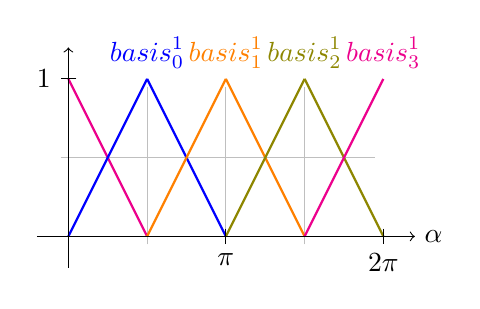
\begin{tikzpicture}
  \draw[color=lightgray] (-0.1, -0.1) grid (3.9, 1.9);

  \draw[thick,color=magenta] (0, 2) -- (1, 0);
  \draw[thick,color=blue] (0, 0) -- (1, 2) node[above] {$\gls{basis}_0^1$};
  \draw[thick,color=blue] (1, 2) -- (2, 0);
  \draw[thick,color=orange] (1, 0) -- (2, 2) node[above] {$\gls{basis}_1^1$};
  \draw[thick,color=orange] (2, 2) -- (3, 0);
  \draw[thick,color=olive] (2, 0) -- (3, 2) node[above] {$\gls{basis}_2^1$};
  \draw[thick,color=olive] (3, 2) -- (4, 0);
  \draw[thick,color=magenta] (3, 0) -- (4, 2) node[above] {$\gls{basis}_3^1$};

  \draw[->] (-0.4, 0) -- (4.4, 0) node[right] {$\alpha$};
  \draw[->] (0, -0.4) -- (0, 2.4);
  \draw (0.1, 2) -- (-0.1, 2) node[left] {$1$};
  \draw (2, 0.1) -- (2, -0.1) node[below] {$\pi$};
  \draw (4, 0.1) -- (4, -0.1) node[below] {$2\pi$};

  \end{tikzpicture}
}
\hspace{1cm}
\subfigure[$K=2$]{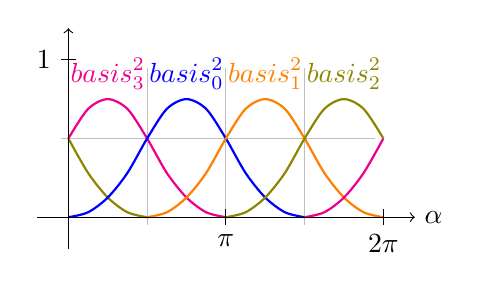
\begin{tikzpicture}
  \draw[color=lightgray] (-0.1, -0.1) grid (3.9, 1.9);

  \draw[color=blue] (1.5,1.5) node[above] {$\gls{basis}_0^2$};
  \draw[color=orange] (2.5,1.5) node[above] {$\gls{basis}_1^2$};
  \draw[color=olive] (3.5,1.5) node[above] {$\gls{basis}_2^2$};
  \draw[color=magenta] (0.5,1.5) node[above] {$\gls{basis}_3^2$};
  \draw[thick,color=magenta] plot [smooth] coordinates {(0,1)(0.25,1.375)(0.5,1.5)(0.75,1.375)(1,1)(1.25,0.5625)(1.5,0.25)(1.75,0.0625)(2,0)};
  \draw[thick,color=olive] plot [smooth] coordinates {(0,1)(0.25,0.5625)(0.5,0.25)(0.75,0.0625)(1,0)};
  \draw[thick,color=blue] plot [smooth] coordinates {(0,0)(0.25,0.0625)(0.5,0.25)(0.75,0.5625)(1,1)(1.25,1.375)(1.5,1.5)(1.75,1.375)(2,1)(2.25,0.5625)(2.5,0.25)(2.75,0.0625)(3,0)};
  \draw[thick,color=orange] plot [smooth] coordinates {(1,0)(1.25,0.0625)(1.5,0.25)(1.75,0.5625)(2,1)(2.25,1.375)(2.5,1.5)(2.75,1.375)(3,1)(3.25,0.5625)(3.5,0.25)(3.75,0.0625)(4,0)};
  \draw[thick,color=olive] plot [smooth] coordinates {(2,0)(2.25,0.0625)(2.5,0.25)(2.75,0.5625)(3,1)(3.25,1.375)(3.5,1.5)(3.75,1.375)(4,1)};
  \draw[thick,color=magenta] plot [smooth] coordinates {(3,0)(3.25,0.0625)(3.5,0.25)(3.75,0.5625)(4,1)};

  \draw[->] (-0.4, 0) -- (4.4, 0) node[right] {$\alpha$};
  \draw[->] (0, -0.4) -- (0, 2.4);
  \draw (0.1, 2) -- (-0.1, 2) node[left] {$1$};
  \draw (2, 0.1) -- (2, -0.1) node[below] {$\pi$};
  \draw (4, 0.1) -- (4, -0.1) node[below] {$2\pi$};

  \end{tikzpicture}
}
\caption[Geschlossene B-Spline-Basisfunktionen]{Illustration geschlossener Basisfunktionen $\gls{basis}_p^K \colon \left(0, 2\pi\right] \to \left[0, 1\right]$ für $P=4$ gleichmäßig verteilter Kontrollpunkte, einmal mit lokaler Kontrollierbarkeit $K=1$ (a) und einmal mit $K=2$ (b).}
\label{fig:bspline}
\end{figure}
